\documentclass[10pt,openany]{book}
\usepackage{ctex}
\usepackage[english]{babel}
\usepackage{amsmath}
\usepackage{amssymb}
\usepackage{tabularx}
\usepackage{graphicx}
\usepackage{algpseudocode}
\usepackage{hyperref}
\usepackage{listings}
\lstdefinestyle{pythonstyle}{language=Python, basicstyle=\ttfamily\small,  commentstyle=\color{gray}, stringstyle=\color{red}, showstringspaces=false, breaklines=true, frame=single}
\usepackage{booktabs}
\usepackage{multirow}
\makeatletter
\newenvironment{breakablealgorithm}
  {% \begin{breakablealgorithm}
   \begin{center}
     \refstepcounter{algorithm}% New algorithm
     \hrule height.8pt depth0pt \kern2pt
     \renewcommand{\caption}[2][\relax]{%
       {\raggedright\textbf{\ALG@name~\thealgorithm} ##2\par}%
       \ifx\relax##1\relax
         \addcontentsline{loa}{algorithm}{\protect\numberline{\thealgorithm}##2}%
       \else
         \addcontentsline{loa}{algorithm}{\protect\numberline{\thealgorithm}##1}%
       \fi
       \kern2pt\hrule\kern2pt
     }
  }{% \end{breakablealgorithm}
     \kern2pt\hrule\relax
   \end{center}
  }
\makeatother
\usepackage{geometry,graphicx,xcolor,color}
\geometry{
  a4paper,
  top=25.4mm, bottom=25.4mm,
  left=20mm, right=20mm,
  headheight=2.17cm,
  headsep=4mm,
  footskip=12mm
}

\usepackage{amssymb,amsmath,mathrsfs}
\usepackage{mathpazo}
\usepackage[nofontspec]{newpxtext}

\definecolor{winered}{rgb}{0.5,0,0}
\definecolor{structurecolor}{RGB}{0, 0, 0}
\definecolor{main}{HTML}{3D445F}
\definecolor{second}{HTML}{627581}
\definecolor{third}{HTML}{9D8798}

\usepackage{hyperref}
\hypersetup{colorlinks = true, linktoc=all, linkcolor=black, urlcolor=winered}

% ------------------------------------------------------------%
% 设置章形式
\usepackage{titlesec, titletoc}
\linespread{1.2} 				
\usepackage{fancyhdr}
\fancyhf{}
\renewcommand{\headrule}{\color{structurecolor}\hrule width\textwidth}
\pagestyle{fancy}
\renewcommand{\headrulewidth}{1pt}
\fancypagestyle{plain}{\renewcommand{\headrulewidth}{0pt}\fancyhf{}\renewcommand{\headrule}{}}

\fancyhead[c]{\color{structurecolor}\kaishu\rightmark}
\fancyfoot[c]{\color{structurecolor}\small\thepage}

\titleformat{\chapter}[display]{\Large}
{\color{structurecolor}\filleft
\parbox{1cm}{\vbox to 1.5cm{\vfill\hbox to 4cm{\hfill\Huge \bfseries \color{structurecolor}{Chapter} \thechapter \hfill}}}}
{1ex}
{\color{structurecolor} \titlerule[2pt]\large\bfseries \filright \vspace*{1em}}
[\vspace*{1em} {\titlerule[2pt]}]

\titleformat{\section}[frame]{\normalfont\color{structurecolor}}{\footnotesize \enspace \large \textcolor{structurecolor}{\S \,\thesection}\enspace}{6pt}{\Large\filcenter \bf \kaishu }

\definecolor{structurecol}{RGB}{0, 178, 238}
\titleformat{\subsection}[hang]{\bfseries}{\large\bfseries\color{structurecol}\thesubsection\enspace}{1pt}{\color{structurecol}\large\bfseries\filright} 

\titleformat{\subsubsection}[hang]{\bfseries}{\large\bfseries\color{structurecolor}\thesubsubsection\enspace}{1pt}{\color{structurecolor}\large\bfseries\filright}
% ------------------------------------------------------------%
% 设置封面
\usepackage{titling}
\renewcommand*{\maketitle}{
    \begin{titlepage}
    \newgeometry{margin = 0in}
    \parindent=0pt
    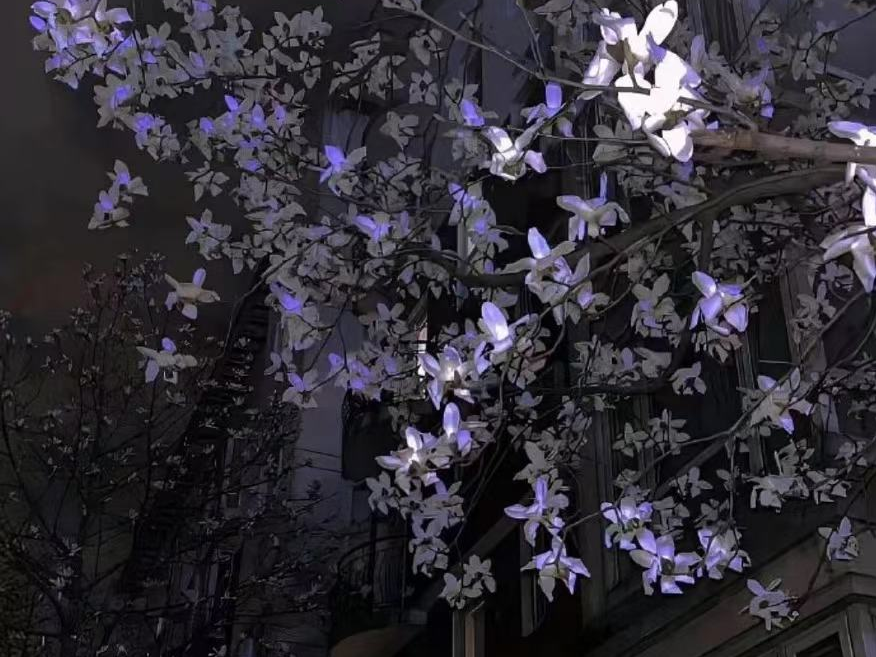
\includegraphics[width=\linewidth]{cover.png}
    \vfill
    \begin{center}
        \parbox{0.618\textwidth}{
        \hfill {\bfseries \Huge \thetitle} \\[0.6pt]  
        \rule{0.618\textwidth}{4pt} \\ 
    }
    \end{center}
    \vfill
    \begin{center}
        \parbox{0.618\textwidth}{
        \hfill\Large
        \kaishu 
          \begin{tabular}{r|}
          作者：\theauthor \\ 
          时间：\thedate \\
        \end{tabular}
        }
    \end{center}
    \vfill
    \begin{center}
        \parbox[t]{0.7\textwidth}{\centering \kaishu }
    \end{center}
    \vfill
\end{titlepage}
\restoregeometry
\thispagestyle{empty}
}
% ------------------------------------------------------------%


\title{LaTeX 文档模板使用说明}
\author{杨彦博}
\date{\today}

\begin{document}
\frontmatter
\maketitle
\tableofcontents
\mainmatter
\songti


\chapter{快速入门}

\section{文档结构}

本模板基于 \texttt{book} 文档类，支持 \textbf{章（chapter）}、\textbf{节（section）}、\textbf{子节（subsection）} 和 \textbf{子子节（subsubsection）} 四个层级。

\subsection{章节命令}

\begin{lstlisting}[style=pythonstyle]
% 创建新的一章
\chapter{章节标题}

% 创建新的一节
\section{小节标题}

% 创建子节
\subsection{子节标题}

% 创建子子节
\subsubsection{子子节标题}
\end{lstlisting}

\subsection{换行与换页}

\begin{lstlisting}[style=pythonstyle]
% 换行（不开始新段落）
这是一行文字。\\ 这是另一行文字。

% 换行并开始新段落（推荐）
这是一段文字。

这是新的一段。

% 强制换页
\newpage

% 分页（允许浮动体优先放置）
\pagebreak
\end{lstlisting}

\section{文字格式}

\subsection{字体样式}

LaTeX 提供了多种\textbf{字体样式}供选择：

\begin{table}[h]
    \centering
    \caption{常用字体样式命令}
    \begin{tabular}{ccc}
    \toprule
        命令 & 效果 & 说明 \\
    \midrule
        \verb|\textbf{文字}| & \textbf{粗体} & 加粗文字 \\
        \verb|\textit{文字}| & \textit{斜体} & 意大利斜体 \\
        \verb|\underline{文字}| & \underline{下划线} & 添加下划线 \\
        \verb|\textcolor{red}{文字}| & \textcolor{red}{红色文字} & 改变颜色 \\
        \verb|\kaishu 文字| & \kaishu 楷书文字 & 楷体（中文） \\
        \verb|\songti 文字| & \songti 宋体文字 & 宋体（中文） \\
    \bottomrule
    \end{tabular}
\end{table}

\subsection{字号设置}

\begin{lstlisting}[style=pythonstyle]
{\tiny 极小字}
{\small 小字}
{\normalsize 正常大小}
{\large 大字}
{\Large 更大字}
{\LARGE 很大字}
{\huge 巨大字}
{\Huge 最大字}
\end{lstlisting}

\subsection{文字颜色}

使用 \verb|xcolor| 宏包定义颜色并使用：

\begin{lstlisting}[style=pythonstyle]
% 在导言区定义颜色
\definecolor{mycolor}{RGB}{255, 0, 0}

% 在正文中使用
\textcolor{mycolor}{这是自定义颜色的文字}

% 预设颜色
\textcolor{red}{红色} \textcolor{blue}{蓝色} \textcolor{green}{绿色}
\end{lstlisting}

\section{列表环境}

\subsection{无序列表}

\begin{lstlisting}[style=pythonstyle]
\begin{itemize}
    \item 第一项
    \item 第二项
    \item 第三项
\end{itemize}
\end{lstlisting}

效果如下：
\begin{itemize}
    \item 第一项
    \item 第二项
    \item 第三项
\end{itemize}

\subsection{有序列表}

\begin{lstlisting}[style=pythonstyle]
\begin{enumerate}
    \item 步骤一
    \item 步骤二
    \item 步骤三
\end{enumerate}
\end{lstlisting}

效果如下：
\begin{enumerate}
    \item 步骤一
    \item 步骤二
    \item 步骤三
\end{enumerate}

\section{插入图片}

\subsection{单张图片}

\begin{lstlisting}[style=pythonstyle]
% 导言区需要：\usepackage{graphicx}

\begin{figure}[h]  % h=here, t=top, b=bottom, p=单独一页
    \centering
    \includegraphics[width=0.6\textwidth]{example.png}
    \caption{这是一张示例图片}
    \label{fig:example}
\end{figure}
\end{lstlisting}

\textbf{常用参数说明：}
\begin{itemize}
    \item \texttt{width=0.6\textbackslash textwidth}：宽度为文本宽度的 60\%
    \item \texttt{height=5cm}：高度为 5 厘米
    \item \texttt{scale=0.8}：缩放为原图的 80\%
    \item \texttt{angle=90}：旋转 90 度
\end{itemize}

\subsection{并排插入多张图片}

\begin{lstlisting}[style=pythonstyle]
\begin{figure}[h]
    \centering
    \begin{minipage}{0.45\textwidth}
        \centering
        \includegraphics[width=\textwidth]{image1.png}
        \caption{图片1说明}
    \end{minipage}
    \hfill
    \begin{minipage}{0.45\textwidth}
        \centering
        \includegraphics[width=\textwidth]{image2.png}
        \caption{图片2说明}
    \end{minipage}
\end{figure}
\end{lstlisting}

\section{插入表格}

\subsection{基本表格}

\begin{lstlisting}[style=pythonstyle]
\begin{table}[h]
    \centering
    \caption{示例表格标题}
    \begin{tabular}{|c|c|c|}
    \hline
    列1 & 列2 & 列3 \\
    \hline
    数据1 & 数据2 & 数据3 \\
    数据4 & 数据5 & 数据6 \\
    \hline
    \end{tabular}
\end{table}
\end{lstlisting}

效果如下：
\begin{table}[h]
    \centering
    \caption{示例表格}
    \begin{tabular}{|c|c|c|}
    \hline
    列1 & 列2 & 列3 \\
    \hline
    数据1 & 数据2 & 数据3 \\
    数据4 & 数据5 & 数据6 \\
    \hline
    \end{tabular}
\end{table}

\subsection{使用 booktabs 的专业表格}

\begin{lstlisting}[style=pythonstyle]
% 导言区需要：\usepackage{booktabs}

\begin{table}[h]
    \centering
    \caption{专业三线表}
    \begin{tabular}{ccc}
    \toprule
        项目 & 数值 & 单位 \\
    \midrule
        速度 & 100 & km/h \\
        高度 & 5000 & m \\
        时间 & 2.5 & h \\
    \bottomrule
    \end{tabular}
\end{table}
\end{lstlisting}

\textbf{列对齐参数：}
\begin{itemize}
    \item \texttt{c}：居中对齐
    \item \texttt{l}：左对齐
    \item \texttt{r}：右对齐
    \item \texttt{p\{3cm\}}：固定宽度 3cm，自动换行
\end{itemize}

\section{插入代码}

\subsection{行内代码}

使用 \verb|\texttt{代码}| 或 \verb|\verb|代码\verb|| 插入行内代码。

示例：使用 \texttt{print("Hello World")} 输出文本。

\subsection{代码块}

\begin{lstlisting}[style=pythonstyle]
% 导言区需要设置：\usepackage{listings}

% Python 代码块
\begin{lstlisting}[style=pythonstyle]
def hello():
    print("Hello, LaTeX!")
    return True
\end{lstlisting}

% 自定义语言和样式
\begin{lstlisting}[language=Python, caption={示例代码}]
import numpy as np
data = np.array([1, 2, 3])
print(data)
\end{lstlisting}

\section{数学公式}

\subsection{行内公式}

使用 \verb|$...$| 插入行内公式，如 $E = mc^2$。

\subsection{独立公式}

\begin{lstlisting}[style=pythonstyle]
% 无编号公式
\[
    \int_{a}^{b} f(x) \, dx
\]

% 有编号公式
\begin{equation}
    \frac{d}{dx} \left( \sin x \right) = \cos x
\end{equation}

% 多行公式
\begin{align}
    a &= b + c \\
    d &= e + f + g
\end{align}
\end{lstlisting}

示例：二次方程求根公式
\begin{equation}
    x = \frac{-b \pm \sqrt{b^2 - 4ac}}{2a}
\label{eq:quadratic}
\end{equation}

公式 \eqref{eq:quadratic} 是二次方程的求根公式。

\section{交叉引用}

\subsection{标签与引用}

\begin{lstlisting}[style=pythonstyle]
% 设置标签
\chapter{引言}\label{ch:intro}
\section{背景}\label{sec:background}
\begin{equation}
    E = mc^2 \label{eq:einstein}
\end{equation}
\begin{figure}[h]
    \includegraphics{example.png}
    \caption{示例图片}\label{fig:example}
\end{figure}
\begin{table}[h]
    \caption{数据表}\label{tab:data}
\end{table}

% 引用
如第~\ref{ch:intro} 章所述...
详见第~\ref{sec:background} 节...
根据公式~\eqref{eq:einstein}...
如图~\ref{fig:example} 所示...
见表~\ref{tab:data}...
\end{lstlisting}

\subsection{引用技巧}

\begin{itemize}
    \item \verb|\ref{label}|：引用编号
    \item \verb|\eqref{label}|：引用公式编号（自动加括号）
    \item \verb|\pageref{label}|：引用所在页码
    \item 在标签前加前缀便于管理：\texttt{ch:}、\texttt{sec:}、\texttt{eq:}、\texttt{fig:}、\texttt{tab:}
\end{itemize}

\section{常用技巧}

\subsection{注释}

\begin{lstlisting}[style=pythonstyle]
% 这是单行注释，不会出现在 PDF 中

% 多行注释可以使用：
\iffalse
这些内容
都不会
出现在 PDF 中
\fi
\end{lstlisting}

\subsection{特殊字符}

\begin{table}[h]
    \centering
    \caption{LaTeX 特殊字符输入方法}
    \begin{tabular}{cc}
    \toprule
        输出 & 输入命令 \\
    \midrule
        \# & \verb|\#| \\
        \$ & \verb|\$| \\
        \% & \verb|\%| \\
        \& & \verb|\&| \\
        \_ & \verb|\_| \\
        \{ \} & \verb|\{ \}| \\
        \textbackslash & \verb|\textbackslash| \\
    \bottomrule
    \end{tabular}
\end{table}

\subsection{间距调整}

\begin{lstlisting}[style=pythonstyle]
% 水平间距
文字\hspace{1cm}文字
文字\quad 文字  % 1em 空格
文字\qquad 文字  % 2em 空格

% 垂直间距
\vspace{1cm}
\smallskip   % 小间距
\medskip     % 中间距
\bigskip     % 大间距
\end{lstlisting}

\chapter{进阶功能}

\section{自定义命令}

在导言区可以定义自己的命令简化写作：

\begin{lstlisting}[style=pythonstyle]
% 在导言区定义
\newcommand{\mycmd}[2]{#1 喜欢 #2}

% 在正文中使用
\mycmd{我}{LaTeX}  % 输出：我喜欢 LaTeX
\end{lstlisting}

\section{文献引用}

\begin{lstlisting}[style=pythonstyle]
% 使用 \cite 命令引用文献
% 详见参考文献 \cite{ref_key}

% 多篇文献引用
% 多项研究\cite{ref1,ref2,ref3}表明...
\end{lstlisting}

\section{超链接}

\begin{lstlisting}[style=pythonstyle]
% 导言区需要：\usepackage{hyperref}

% 网页链接
\href{https://www.example.com}{示例网站}

% 邮箱链接
\href{mailto:example@email.com}{发送邮件}

% 显示 URL
\url{https://www.example.com}
\end{lstlisting}

\section{编译注意事项}

\begin{enumerate}
    \item \textbf{首次编译}：需要编译两次以生成正确的目录和交叉引用
    \item \textbf{使用 XeLaTeX}：支持中文的最佳编译方式
    \item \textbf{图片格式}：推荐使用 PNG、JPG 或 PDF 格式
    \item \textbf{文件编码}：确保 \texttt{.tex} 文件为 UTF-8 编码
\end{enumerate}

\end{document}